\documentclass[main.tex]{subfiles}

\begin{document}

\appendix
\section{Bilaga. VHDL-kod}
\subfile{sections/appendices/opdec}

\newpage
% set landscape
\KOMAoptions{paper={landscape},pagesize}
\recalctypearea
\vspace*{-10mm}
\section{Bilaga. Blockscheman}
\subsection{Huvudhierarki}
\label{diag:comp}
\begin{minipage}{\textwidth}
    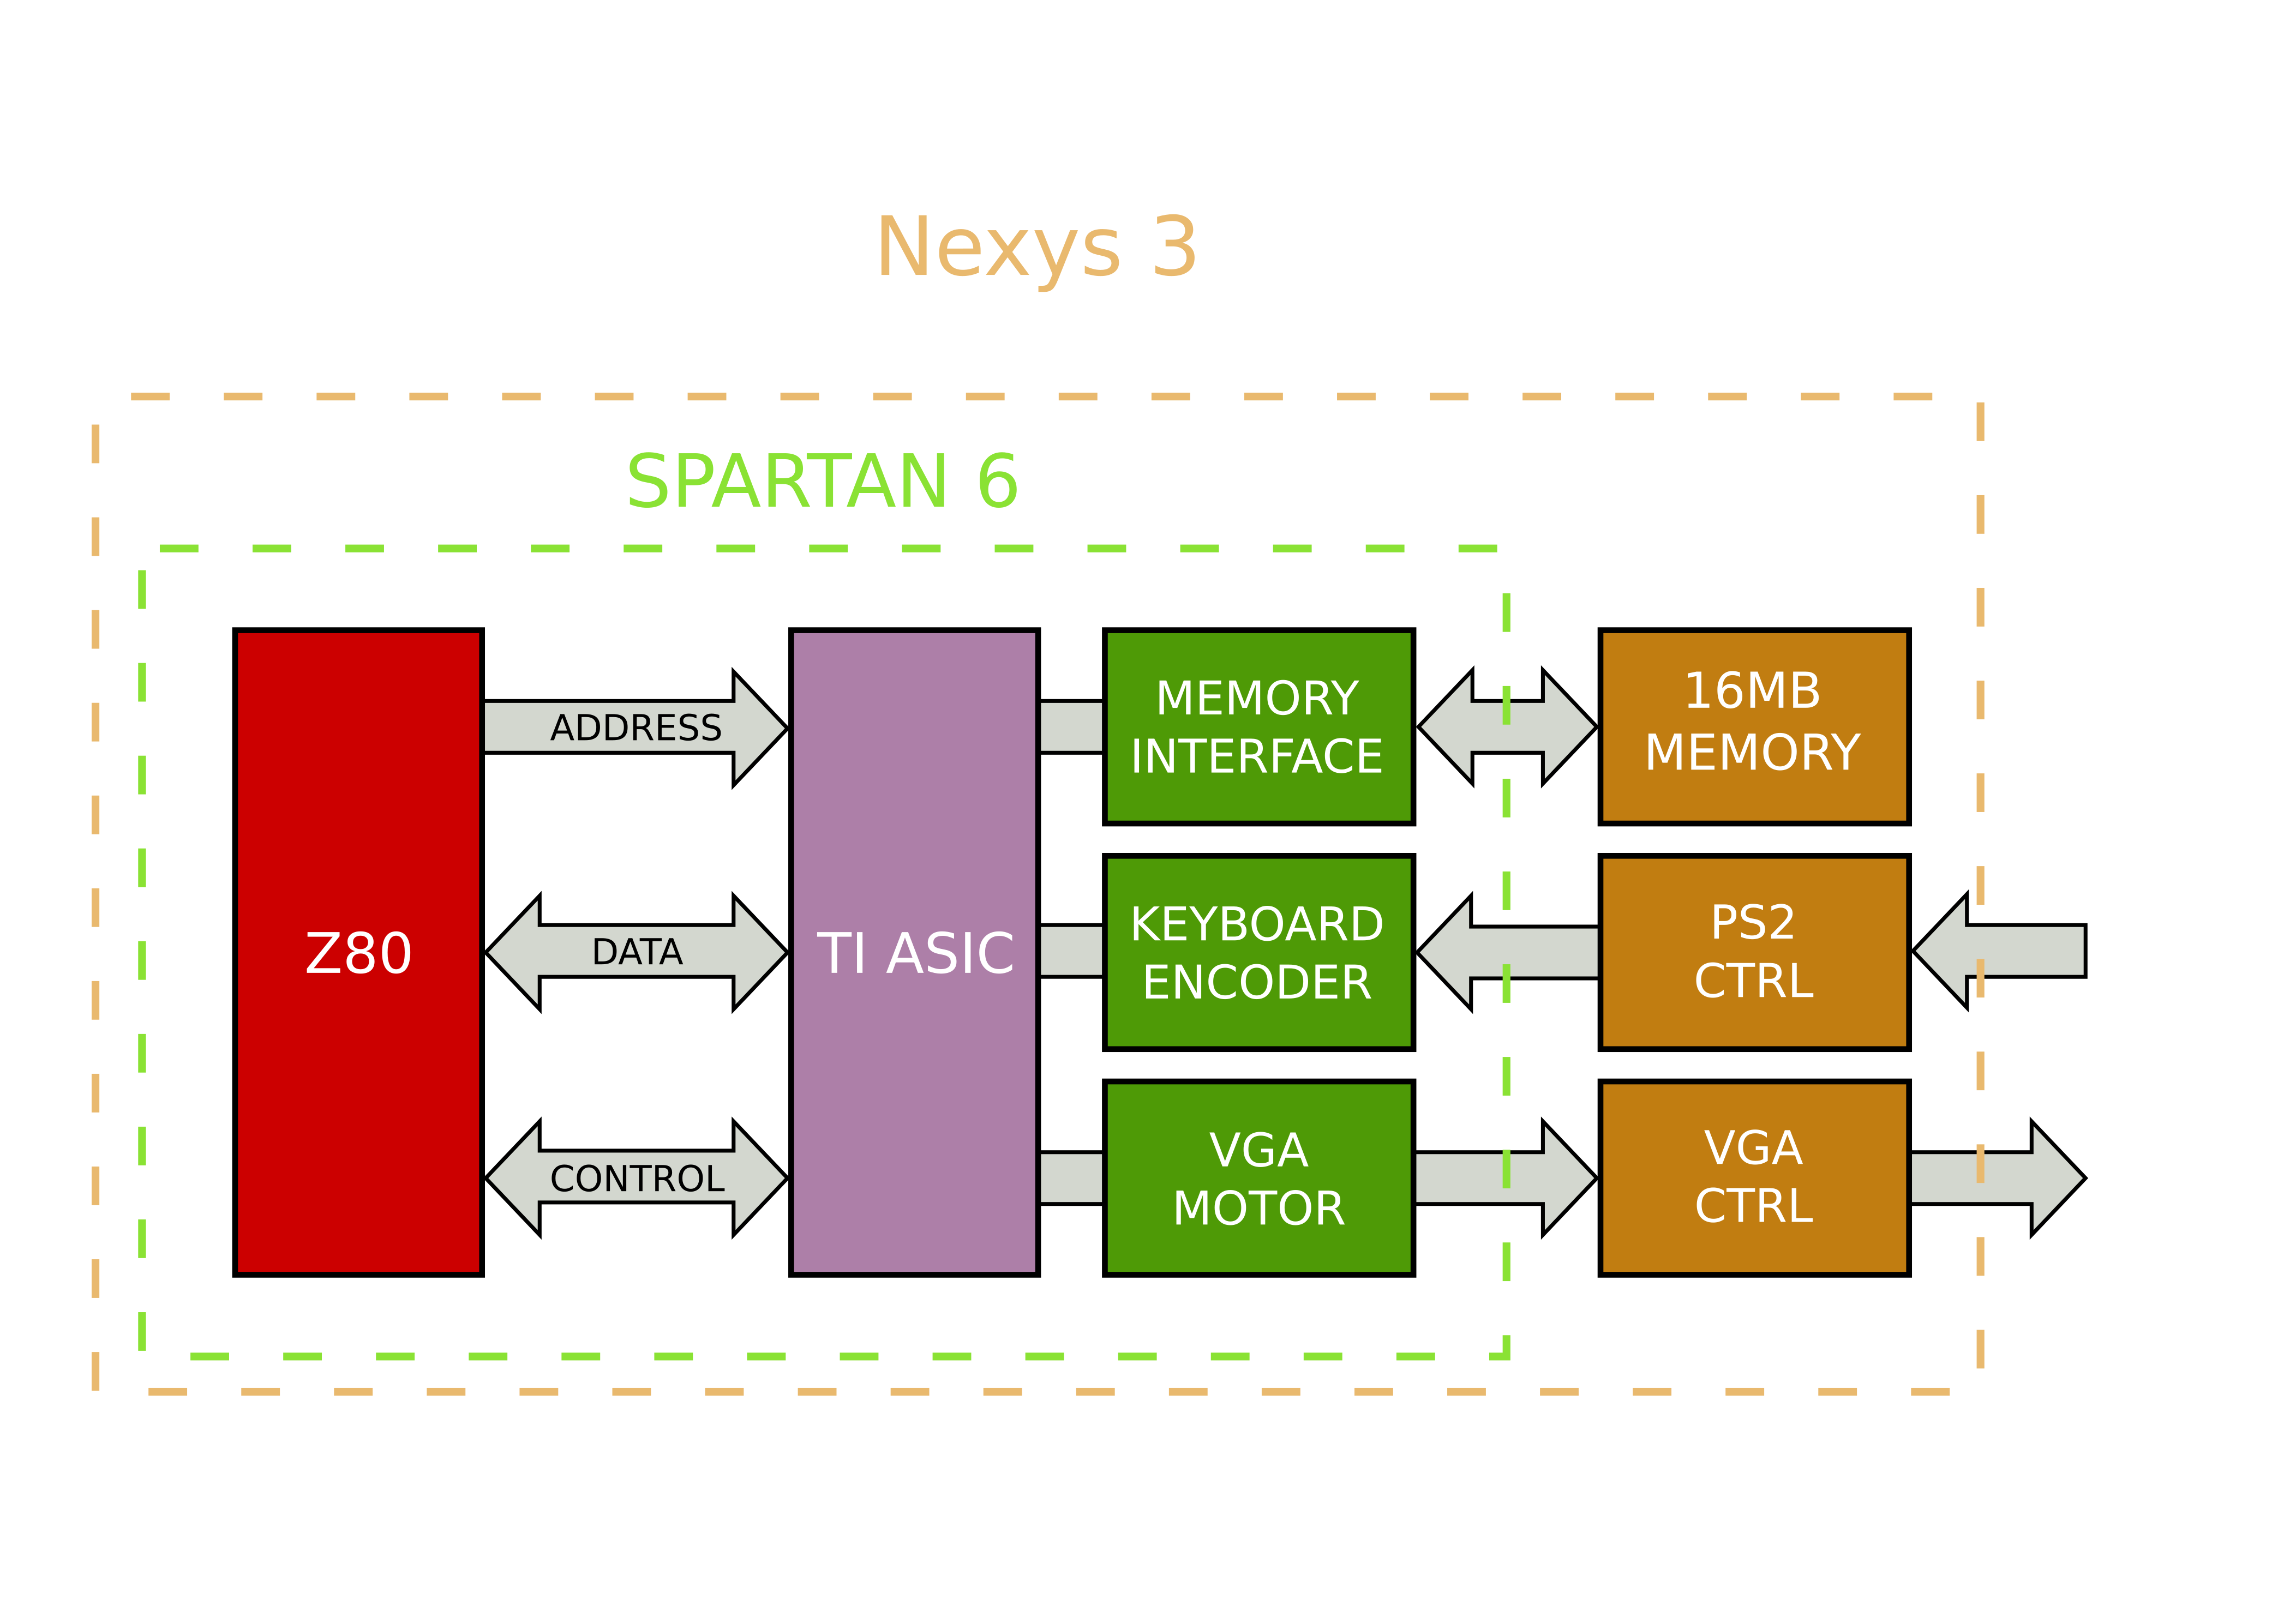
\includegraphics[scale=0.80]{comp.eps}
\end{minipage}
\vspace*{-10mm}
\subsection{Z80}
\label{diag:z80}
\begin{minipage}{\textwidth}
    \vspace{-2mm}
    \hspace{-15mm}
    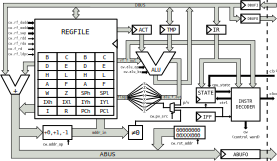
\includegraphics[scale=0.90]{cpu.eps}
\end{minipage}
\vspace*{-10mm}
\subsection{ALU}
\label{diag:alu}
\begin{minipage}{\textwidth}
    \includegraphics[scale=0.71]{alu.eps}
\end{minipage}
\vspace*{-10mm}
\subsection{TI-ASIC}
\label{diag:ti}
\begin{minipage}{\textwidth}
    \includegraphics[scale=0.80]{ti.eps}
\end{minipage}
\newpage
% set portrait
\KOMAoptions{paper={landscape},pagesize}
\recalctypearea
\end{document}
